\documentclass[10pt,twocolumn,a4paper]{article}
\usepackage[margin=1.8cm]{geometry}
\usepackage{amsmath,amssymb,bm}
\usepackage{graphicx,booktabs,caption}
\usepackage[hidelinks]{hyperref}
\usepackage{lmodern}
\usepackage[T1]{fontenc}
\usepackage{microtype}
\usepackage{xcolor}
\usepackage{abstract}
\captionsetup{font=small,labelfont=bf}
\setlength{\abovecaptionskip}{4pt}
\setlength{\columnsep}{0.7cm}
% let floats fill more of each page, so they do not spill onto trailing float-only pages
\renewcommand{\topfraction}{0.92}
\renewcommand{\bottomfraction}{0.7}
\renewcommand{\textfraction}{0.07}
\renewcommand{\floatpagefraction}{0.75}
\renewcommand{\dbltopfraction}{0.92}
\renewcommand{\dblfloatpagefraction}{0.75}
\setcounter{topnumber}{3}
\setcounter{bottomnumber}{2}
\setcounter{totalnumber}{5}
\setcounter{dbltopnumber}{3}
\newcommand{\NL}{63}
\newcommand{\Mtrain}{29\,312}
\newcommand{\Mtest}{7\,401}
\newcommand{\Mnovel}{7401}
\newcommand{\Mcopies}{0}
\newcommand{\PctCopies}{0}
\newcommand{\ThetaTrain}{0.312}
\newcommand{\MeffTrain}{3590}
\newcommand{\ThetaTest}{0.303}
\newcommand{\MeffTest}{1280}
\newcommand{\MeffNovel}{1280}
\newcommand{\NfOne}{1\,323}
\newcommand{\NCij}{861\,273}
\newcommand{\Hbest}{128}
\newcommand{\dbest}{10}
\newcommand{\lambest}{10^{-3}}
\newcommand{\Nparams}{217\,728}
\newcommand{\BestEpoch}{668}
\newcommand{\ValNLPL}{82.18}
\newcommand{\NLPLtrain}{71.10}
\newcommand{\NLPLtest}{78.72}
\newcommand{\NLPLnovel}{78.72}
\newcommand{\NLPLgap}{7.6}
\newcommand{\NLPLgapPct}{11}
\newcommand{\NLPLtestSite}{1.25}
\newcommand{\PPVL}{0.83}
\newcommand{\PPVLhalf}{1.00}
\newcommand{\PPVbase}{0.21}
\newcommand{\PCone}{11.3}
\newcommand{\PCtwo}{4.3}
\newcommand{\Etest}{-131.7}
\newcommand{\Etrain}{-134.3}
\newcommand{\Erandom}{-0.0}
\newcommand{\HamTestTest}{0.60}
\newcommand{\HamTestNN}{0.12}
\newcommand{\HamNovelTrain}{0.18}
\newcommand{\HamTestTrain}{0.18}
\newcommand{\rCtrain}{0.944}
\newcommand{\rCprof}{-0.005}
\newcommand{\sCtrain}{0.88}
\newcommand{\Crel}{0.94}
\newcommand{\sCdisTrain}{0.94}
\newcommand{\sCdisOne}{0.83}
\newcommand{\sCdisStar}{0.91}
\newcommand{\rCnovelFull}{1.000}
\newcommand{\BetaStar}{1.05}
\newcommand{\TauOne}{6.5}
\newcommand{\TauPOne}{3.8}
\newcommand{\BurnOne}{500}
\newcommand{\NgenOne}{10\,000}
\newcommand{\NcolOne}{0}
\newcommand{\PctColOne}{0.0}
\newcommand{\StudyColNatOne}{0.0}
\newcommand{\StudyColRndOne}{0.0}
\newcommand{\HamEndOne}{0.66}
\newcommand{\SweepsNinetyOne}{11}
\newcommand{\EendNatOne}{-126.6}
\newcommand{\EendRndOne}{-126.6}
\newcommand{\EgenOne}{-125.9}
\newcommand{\rFOne}{0.990}
\newcommand{\rCOne}{0.871}
\newcommand{\sCOne}{0.78}
\newcommand{\rCnovelOne}{0.871}
\newcommand{\HamGGOne}{0.68}
\newcommand{\HamGTOne}{0.44}
\newcommand{\HamGTrOne}{0.42}
\newcommand{\HamGTrMinOne}{0.32}
\newcommand{\UniqOne}{100.0}
\newcommand{\StudySweeps}{2000}
\newcommand{\WPCaOne}{0.26}
\newcommand{\WPCbOne}{0.34}
\newcommand{\WEOne}{5.9}
\newcommand{\TauStar}{5.6}
\newcommand{\TauPStar}{3.4}
\newcommand{\BurnStar}{500}
\newcommand{\NgenStar}{10\,000}
\newcommand{\NcolStar}{0}
\newcommand{\PctColStar}{0.0}
\newcommand{\StudyColNatStar}{0.0}
\newcommand{\StudyColRndStar}{0.0}
\newcommand{\HamEndStar}{0.64}
\newcommand{\SweepsNinetyStar}{17}
\newcommand{\EendNatStar}{-134.6}
\newcommand{\EendRndStar}{-134.6}
\newcommand{\EgenStar}{-133.8}
\newcommand{\rFStar}{0.992}
\newcommand{\rCStar}{0.859}
\newcommand{\sCStar}{0.85}
\newcommand{\rCnovelStar}{0.859}
\newcommand{\HamGGStar}{0.65}
\newcommand{\HamGTStar}{0.41}
\newcommand{\HamGTrStar}{0.39}
\newcommand{\HamGTrMinStar}{0.29}
\newcommand{\UniqStar}{100.0}
\newcommand{\WPCaStar}{0.30}
\newcommand{\WPCbStar}{0.31}
\newcommand{\WEStar}{2.1}
\newcommand{\WPCaTrain}{1.23}
\newcommand{\WPCbTrain}{0.29}
\newcommand{\WPCaProf}{1.05}
\newcommand{\WPCbProf}{0.66}
\newcommand{\WEtrain}{2.7}
\newcommand{\WEprof}{39.5}
\newcommand{\Eunw}{-146.2}
\newcommand{\ClTest}{14.1}
\newcommand{\ClTrain}{12.9}
\newcommand{\ClOne}{5.1}
\newcommand{\ClStar}{3.2}
\newcommand{\Kclust}{3}
\newcommand{\NcovClust}{2}
\newcommand{\CovWeight}{85.9}
\newcommand{\NtestCov}{6\,761}
\newcommand{\MeffTestCov}{1102}
\newcommand{\rCtrainCov}{0.941}
\newcommand{\rFcovOne}{0.991}
\newcommand{\rCcovOne}{0.918}
\newcommand{\sCcovOne}{0.82}
\newcommand{\rCcovTopOne}{0.961}
\newcommand{\rFcovStar}{0.996}
\newcommand{\rCcovStar}{0.918}
\newcommand{\sCcovStar}{0.91}
\newcommand{\rCcovTopStar}{0.961}
\newcommand{\NsuperSet}{36\,713}
\newcommand{\OrigCopies}{78.8}
\newcommand{\OrigNN}{0.044}
\newcommand{\SplitThresh}{0.2}
\newcommand{\SplitIdent}{80}
\newcommand{\NclustTot}{10\,942}
\newcommand{\NsingleClust}{6\,767}
\newcommand{\NtrainClean}{29\,312}
\newcommand{\NtestClean}{7\,401}
\newcommand{\NdropClean}{0}
\newcommand{\CleanNN}{0.179}
\newcommand{\CleanNNmin}{0.016}
\newcommand{\CleanNNminSub}{1}
\newcommand{\CleanNNmed}{0.175}
\newcommand{\CleanNNqfive}{0.032}
\newcommand{\CleanPctNear}{61}
\newcommand{\CleanDropRule}{exact}
\newcommand{\CmpMtrain}{14\,502}
\newcommand{\CmpMtest}{3\,739}
\newcommand{\CmpPctCopies}{79}
\newcommand{\CmpValNLPL}{85.61}
\newcommand{\CmpNLPLtest}{75.70}
\newcommand{\CmpNLPLnovel}{77.13}
\newcommand{\CmprFOne}{0.990}
\newcommand{\CmprCOne}{0.865}
\newcommand{\CmprCtrain}{0.960}
\newcommand{\CmpHamGTrOne}{0.42}
\newcommand{\CmpPPVLhalf}{0.97}
\newcommand{\CmprCcovOne}{0.921}
\newcommand{\MissCl}{C0}
\newcommand{\EmissTest}{-119.5}
\newcommand{\EmissTrain}{-122.6}
\newcommand{\EcovTest}{-134.0/-133.5}
\newcommand{\EcovTrain}{-134.5/-137.2}
\newcommand{\EgapMiss}{14}
\newcommand{\PLLmissTrain}{-71.8}
\newcommand{\PLLcovTrain}{-71.1/-71.0}
\newcommand{\dFmiss}{+1.01}
\newcommand{\dFmissFac}{0.36}


\title{\vspace{-1.2cm}\large\bfseries Generative modelling of the bacterial J-domain family with
an attention-parametrised Potts model}
\author{\normalsize TP4 --- AttentionDCA}
\date{\normalsize\today}

\begin{document}
\twocolumn[
\begin{@twocolumnfalse}
\maketitle
\begin{abstract}
\noindent
We fit a Potts model of the bacterial J-domain family ($L=\NL$, $q=21$) whose coupling tensor is
parametrised by a factored self-attention layer, train it by maximising the reweighted
pseudo-likelihood, and sample new sequences from the learned conditionals. Since the supplied
train/test split repeats \CmpPctCopies\% of its sequences verbatim across the two sides, we work
throughout on a sequence-disjoint split rebuilt from the full
\NsuperSet-sequence pool. On it the model reaches a held-out pseudo-likelihood
\NLPLgapPct\% above its training value and recovers \PPVLhalf\ precision on the top $L/2$ structural
contacts. Sequences generated by the pseudo-likelihood sampler reproduce the natural one-site
frequencies ($r=\rFOne$) and connected two-site correlations ($r=\rCOne$, against a train-vs-test
ceiling of $\rCtrain$), are new (mean distance \HamGTrOne\ to the closest training sequence,
against \HamTestTrain\ for natural held-out sequences) and as diverse as natural sequences
(\HamGGOne\ vs.\ \HamTestTest\ mean pairwise distance). Chains decorrelate from their seed in
\SweepsNinetyOne\ sweeps ($\tau_\text{int}=\TauOne$). The one systematic failure is a minor
HscB-like sub-family carrying \ClTest\% of the natural weight but only \ClOne\% of the samples;
restricting the comparison to the modes the sampler does populate raises the correlation agreement
to $\rCcovOne$ against a $\rCtrainCov$ ceiling. That sub-family is not mis-modelled but
mis-weighted: its conditionals are fitted as well as any other cluster's, while its energy sits
\EgapMiss\ units too high --- pseudo-likelihood constrains conditionals, never the relative masses
of the basins, so the model learns each sub-family but not the prior over them.
\vspace{0.5cm}
\end{abstract}
\end{@twocolumnfalse}
]

%======================================================================
\section{Introduction}
%======================================================================
Direct Coupling Analysis models a protein family as a Potts distribution over aligned sequences,
\begin{equation}
P(\bm x)=\tfrac1Z e^{-E(\bm x)},\qquad E(\bm x)=-\sum_{i<j}J_{ij}(x_i,x_j),
\label{eq:potts}
\end{equation}
whose couplings $J_{ij}(a,b)$ encode the co-evolution between positions. Fitting a full coupling
tensor means $\binom{L}{2}q^2$ parameters, which for $L=\NL$, $q=21$ is $861\,273$ numbers
estimated from a few thousand effectively independent sequences.

AttentionDCA replaces that tensor by a factored attention layer. With $H$ heads carrying
query/key matrices $Q^h,K^h\in\mathbb R^{d\times L}$ and a value matrix $V^h\in\mathbb R^{q\times q}$,
\begin{align}
A^h_{ij}&=\operatorname{softmax}_j\big(\textstyle\sum_k Q^h_{ki}K^h_{kj}\big),\quad A^h_{ii}=0,\\
J_{ij}(a,b)&=\sum_{h=1}^{H}A^h_{ij}\,V^h(a,b),
\label{eq:att}
\end{align}
which separates \emph{which} positions interact ($A^h$) from the amino-acid chemistry of the
interaction ($V^h$) and costs only $H(2dL+q^2)$ parameters. Following the original formulation no
explicit fields are used: conservation is absorbed into the couplings.

This work has three aims: to train that model on the J-domain family by pseudo-likelihood, to
sample new sequences from it and to ask, quantitatively, in what respects those sequences do and
do not look like natural ones.

%======================================================================
\section{Methods}
%======================================================================
\paragraph{Pseudo-likelihood training.} $Z$ in Eq.~\eqref{eq:potts} is intractable, so we maximise
the pseudo-likelihood built from the exact single-site conditionals
\begin{equation}
p(x_i=a\mid\bm x_{\setminus i})=\frac{\exp\sum_{j\neq i}J_{ij}(a,x_j)}
{\sum_c\exp\sum_{j\neq i}J_{ij}(c,x_j)},
\label{eq:cond}
\end{equation}
minimising $\mathcal L=-\sum_m w_m\sum_i\log p(x^m_i\mid\bm x^m_{\setminus i})
+\lambda\sum_{i\neq j,a,b}J_{ij}(a,b)^2$ with Adam (lr $5\cdot10^{-3}$, batches of 1000), a 10\%
validation split and early stopping on the validation pseudo-likelihood.

\paragraph{Reweighting.} Natural alignments over-represent well-sampled clades, so each sequence
carries $w_m=1/|\{n: d_H(\bm x^m,\bm x^n)<\theta L\}|$ with
$\theta=\min(0.5,\,0.38\cdot0.32/\langle\text{fraction identity}\rangle)$, giving
$M_\text{eff}=\sum_m w_m$. The same weights are used for every natural statistic reported below;
generated sets are weighted uniformly.

\paragraph{Sampling.} New sequences are drawn with the learned conditionals: one \emph{sweep}
visits the $L$ sites in random order and resamples each from Eq.~\eqref{eq:cond} raised to an
inverse temperature $\beta$. Since $A^h$ is row-normalised, $J_{ij}\neq J_{ji}^\top$ and the chain
is only approximately Boltzmann; we therefore monitor both the symmetrised Hamiltonian
$E(\bm x)=-\frac12\sum_{i\neq j}J_{ij}(x_i,x_j)$ and the pseudo-log-likelihood
$\log\mathrm{PL}(\bm x)=\sum_i\log p(x_i\mid\bm x_{\setminus i})$. All chains are advanced
simultaneously on the GPU, which costs ${\sim}0.3\,\mu$s per chain-update against
0.6--28\,ms for the original per-site Python loop.

\paragraph{Metrics.} We compare weighted one- and two-site statistics
$f_i(a)$, $f_{ij}(a,b)$ and $C_{ij}(a,b)=f_{ij}(a,b)-f_i(a)f_j(b)$ entry-wise, using the Pearson
$r$ (tightness of the relation) and the least-squares slope of generated on natural (amplitude;
the two are linked by $\text{slope}=r\,\sigma_\text{gen}/\sigma_\text{nat}$). Novelty and diversity
use the normalised Hamming distance $d(\bm x,\bm y)=\frac1L\sum_i(1-\delta_{x_i,y_i})$.
Two references bracket every number: \emph{train vs.\ test}, the finite-sample ceiling, and an
\emph{independent-site} model sampled from the training $f_i$, which matches $f_i$ by construction
and has $C_{ij}\equiv0$.

\paragraph{Data and split.} An audit of the alignments shipped with the project showed that its
train/test pair is species-disjoint but not sequence-disjoint: \OrigCopies\% of the test sequences
are byte-identical to a training sequence, because the same J-domain recurs across species. We
therefore build the split from the full \NsuperSet-sequence pool by clustering greedily
(CD-HIT style, \SplitIdent\% identity, \NclustTot\ clusters) and assigning whole clusters to one
side, removing afterwards only sequences identical to a training one. This gives \Mtrain\ training
and \Mtest\ test sequences with no exact copies (median distance to the nearest training sequence
\CleanNNmed). Test sequences that merely \emph{resemble} training ones are kept --- discarding
them would leave only the isolated corners of the family and misrepresent the density the
generative model must reproduce. The companion report documents the audit in full.

\paragraph{Units.} Log-likelihoods use the natural logarithm and are quoted in \emph{nats}
($1$ nat $=1/\ln2\approx1.44$ bits): a difference of $\Delta$ nats means one model assigns the
data $e^\Delta$ times more probability, so $0.7$ nats is a factor of two.

%======================================================================
\section{Results}
%======================================================================

\subsection{Training and structural validation}
A grid over $H$, $d$ and $\lambda$ scored by validation pseudo-likelihood
(Table~\ref{tab:sweep}) selects $H=\Hbest$, $d=\dbest$, $\lambda=\lambest$ (\Nparams\
parameters). Performance improves with head count up to ${\sim}128$ heads and then saturates:
doubling to 256 buys $0.3$ nats per sequence for twice the parameters.

The fitted model attains \NLPLtrain\ nats per sequence on training data and \NLPLtest\ on the
held-out set (Fig.~\ref{fig:train}). Because that test set shares no sequence with the training
set, the \NLPLgapPct\% difference is a genuine generalisation gap. On the supplied split the same
quantity is almost flat (\CmpNLPLtest\ vs.\ \CmpValNLPL), which is exactly what one expects when
most ``held-out'' sequences were in fact seen.

That the couplings are physically meaningful, and not merely predictive, is confirmed
independently of any generation: after symmetrisation, zero-sum gauge, Frobenius norm and average
product correction, the top-ranked long-range pairs ($|i-j|>4$) are true contacts ($<8$\,\AA) with
precision \PPVLhalf\ at $L/2$ pairs and \PPVL\ at $L$ pairs, against a \PPVbase\ base rate.

\begin{figure*}[t]\centering
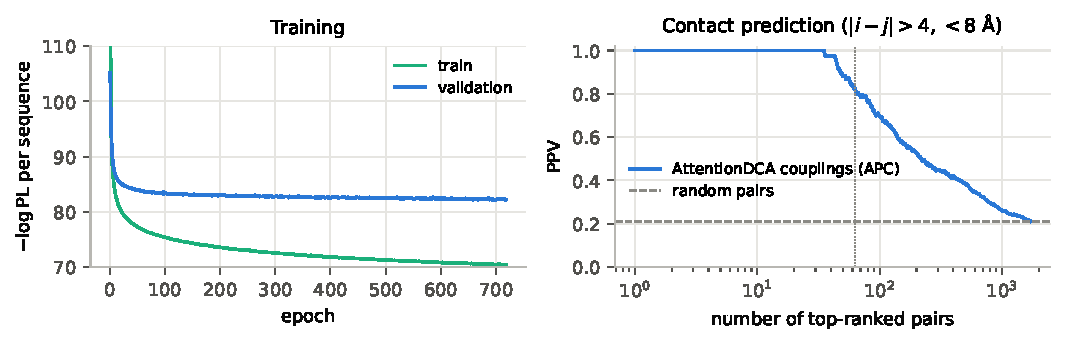
\includegraphics[width=0.86\textwidth]{../outputs/figures/training_contacts_clean.pdf}
\caption{Left: weighted $-\log\mathrm{PL}$ per sequence. Right: contact-prediction precision of the
ranked APC-corrected coupling norms; vertical line at $L$ pairs.}
\label{fig:train}
\end{figure*}

\begin{table}[t]\centering\small
\begin{tabular}{rrlrrr}
\toprule
$H$ & $d$ & $\lambda$ & params & best epoch & val.\ $-\log\mathrm{PL}$ \\
\midrule
256 & 10 & $10^{-3}$ & 435\,456 & 187 & 85.33 \\
128 & 10 & $10^{-3}$ & 217\,728 & 387 & 85.61 \\
64 & 10 & $10^{-3}$ & 108\,864 & 709 & 86.73 \\
64 & 10 & $10^{-4}$ & 108\,864 & 168 & 87.34 \\
64 & 23 & $10^{-4}$ & 213\,696 & 293 & 87.37 \\
64 & 23 & $10^{-3}$ & 213\,696 & 654 & 87.63 \\
32 & 10 & $10^{-4}$ & 54\,432 & 817 & 87.78 \\
32 & 23 & $10^{-4}$ & 106\,848 & 697 & 88.17 \\
32 & 23 & $10^{-3}$ & 106\,848 & 2061 & 88.22 \\
32 & 10 & $10^{-3}$ & 54\,432 & 817 & 89.10 \\
16 & 10 & $10^{-4}$ & 27\,216 & 973 & 89.74 \\
16 & 23 & $10^{-4}$ & 53\,424 & 820 & 90.61 \\
16 & 23 & $10^{-3}$ & 53\,424 & 2024 & 90.64 \\
16 & 10 & $10^{-3}$ & 27\,216 & 1692 & 91.34 \\
\bottomrule
\end{tabular}
\caption{Hyper-parameter grid sorted by validation $-\log\mathrm{PL}$ per sequence. The chosen
model is the second row.}
\label{tab:sweep}
\end{table}

\subsection{The sampler mixes, and needs a temperature}
Chains started from natural training sequences and from uniform random sequences converge to the
same stationary energy (\EendNatOne\ vs.\ \EendRndOne\ at $\beta=1$), so the stationary state does
not depend on the initialisation (Fig.~\ref{fig:mixing}). The distance to the seed reaches 90\% of
its plateau after \SweepsNinetyOne\ sweeps, and the plateau (\HamEndOne) matches the mean
test--test distance: the chain forgets its starting sequence entirely. The integrated
autocorrelation time of the energy is $\tau_\text{int}=\TauOne$ sweeps. We generate \NgenOne\
sequences per temperature, each the final state of an independent chain run for \BurnOne\ sweeps
($\approx40\,\tau_\text{int}$). No chain ends in a degenerate gap-only state.

Pseudo-likelihood constrains the conditionals but not the global normalisation, so $\beta=1$ need
not reproduce the energy scale of natural sequences. Figure~\ref{fig:beta} scans $\beta$: raising
it deepens the energy and sharpens the correlations at the cost of diversity. We report both
$\beta=1$, the learned model as it stands, and $\beta^*=\BetaStar$, defined by matching the mean
sample energy to the reweighted mean energy of the \emph{training} set --- a criterion that never
touches the test set.

\begin{figure}[!htb]\centering
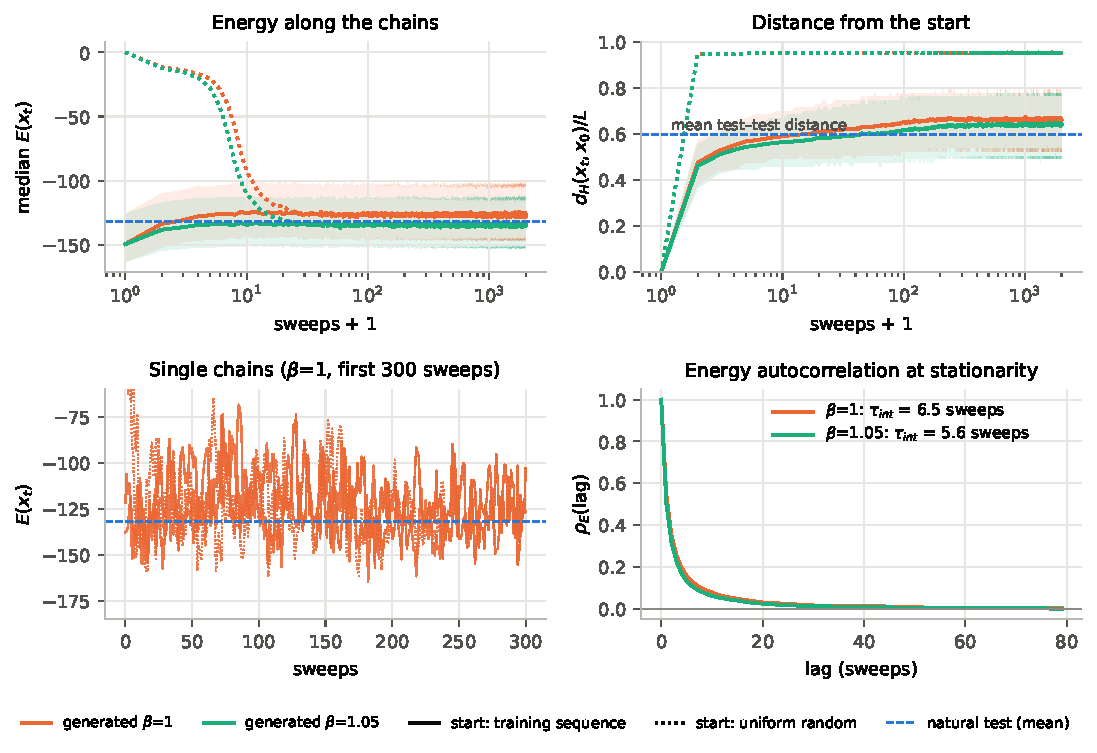
\includegraphics[width=\linewidth]{../outputs/figures/mixing_clean.pdf}
\caption{Pseudo-likelihood sampling. (a) median energy (band: 10--90\% of chains from training
starts); (b) Hamming distance to the starting sequence; (c) individual chains at $\beta=1$;
(d) chain-averaged energy autocorrelation at stationarity.}
\label{fig:mixing}
\end{figure}

\begin{figure*}[t]\centering
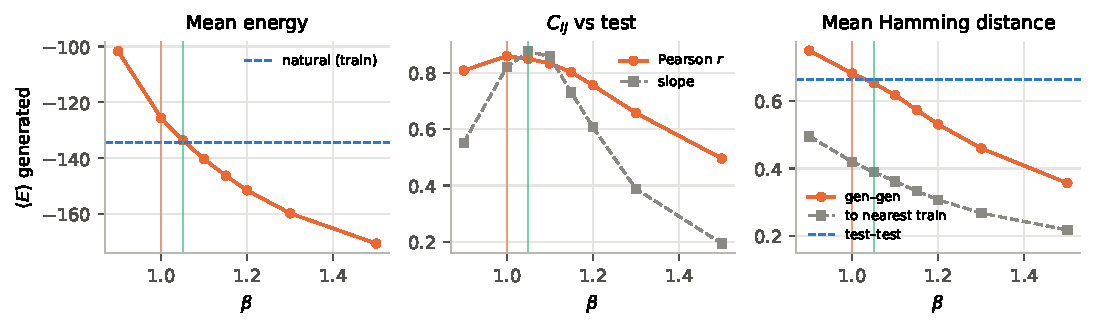
\includegraphics[width=0.86\textwidth]{../outputs/figures/beta_scan_clean.pdf}
\caption{Inverse-temperature scan (chains started from training sequences). Vertical lines mark
$\beta=1$ and $\beta^*=\BetaStar$.}
\label{fig:beta}
\end{figure*}

\subsection{One- and two-site statistics}
Site frequencies are reproduced almost exactly ($r=\rFOne$ at $\beta=1$, $\rFStar$ at $\beta^*$),
but so are they by the independent-site baseline, so the informative quantity is the connected
correlation. There the model reaches $r=\rCOne$ ($\beta=1$) and $\rCStar$ ($\beta^*$) against a
finite-sample ceiling of $\rCtrain$ and a baseline of $\rCprof$ (Fig.~\ref{fig:stats},
Table~\ref{tab:stats}).

The regression slope separates two different errors. Since
$\text{slope}=r\,\sigma_\text{gen}/\sigma_\text{nat}$, it reports amplitude where $r$ reports
tightness. At $\beta=1$ the slope is $\sCOne$: the model identifies the right correlations but
systematically \emph{under-states} them, its samples being under-dispersed. At $\beta^*$ it rises
to $\sCStar$, against a train-vs-test ceiling of $\sCtrain$.

That the ceiling is itself below 1 is regression dilution: the natural $C_{ij}$ are estimated from
only $M_\text{eff}=\MeffTest$ effective sequences, and noise in the predictor biases any
least-squares slope towards zero. Correlating two independent halves of the test set and applying
the Spearman--Brown formula puts the reliability of the natural $C_{ij}$ at \Crel; dividing through
by it gives disattenuated slopes of \sCdisOne\ ($\beta=1$), \sCdisStar\ ($\beta^*$) and
\sCdisTrain\ (ceiling). Read against that ceiling rather than against 1, $\beta^*$ recovers the
correlation amplitude to within a few percent, while $\beta=1$ falls short by about 10\%. The
ceiling does not reach 1 because clustering sends whole groups to one side, so train and test
sample somewhat different regions of the family.

\begin{figure*}[t]\centering
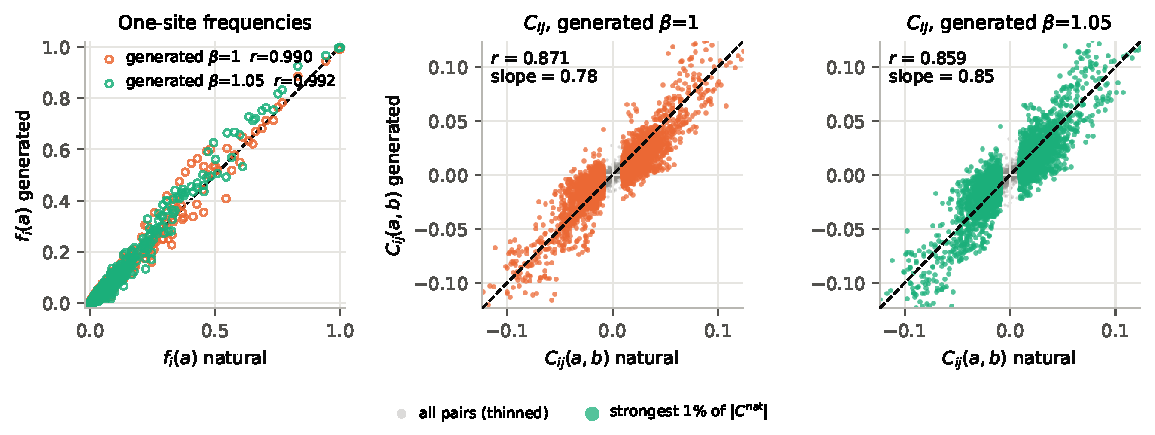
\includegraphics[width=0.86\textwidth]{../outputs/figures/freqs_corr_clean.pdf}
\caption{Generated vs.\ natural (reweighted test) one-site frequencies and connected
correlations. The $C_{ij}$ panels show the strongest 1\% of $|C^\text{nat}|$ in colour over a
thinned grey sample of all \NCij\ entries. Dashed: identity.}
\label{fig:stats}
\end{figure*}

\begin{table*}[t]\centering\small\setlength{\tabcolsep}{4pt}
\begin{tabular}{llcccc}
\toprule
statistic & set vs.\ natural test & Pearson $r$ & Spearman $\rho$ & slope & RMSE \\
\midrule
$f_i(a)$ & generated, $\beta=1$ & 0.990 & 0.972 & 1.01 & 0.0160 \\
 & generated, $\beta^*=1.05$ & 0.992 & 0.970 & 1.06 & 0.0165 \\
 & natural train (ceiling) & 0.998 & 0.983 & 0.99 & 0.0070 \\
 & independent-site model & 0.998 & 0.982 & 0.99 & 0.0072 \\
\midrule
$C_{ij}(a,b)$ & generated, $\beta=1$ & 0.871 & 0.193 & 0.78 & 0.0015 \\
 & generated, $\beta^*=1.05$ & 0.859 & 0.209 & 0.85 & 0.0016 \\
 & natural train (ceiling) & 0.944 & 0.377 & 0.88 & 0.0010 \\
 & independent-site model & -0.005 & 0.058 & -0.00 & 0.0030 \\
\midrule
$C_{ij}$, top 1\% & generated, $\beta=1$ & 0.918 & 0.880 & 0.84 & 0.0113 \\
 & generated, $\beta^*=1.05$ & 0.908 & 0.865 & 0.93 & 0.0123 \\
 & natural train (ceiling) & 0.981 & 0.949 & 0.91 & 0.0057 \\
 & independent-site model & -0.009 & -0.022 & -0.00 & 0.0283 \\
\bottomrule
\end{tabular}
\caption{Agreement with the natural test set (natural sets reweighted, generated uniform).
``Top 1\%'': the 1\% largest $|C^\text{test}_{ij}(a,b)|$.}
\label{tab:stats}
\end{table*}

\subsection{A missing sub-family, and what it costs}
Projected on the first two principal components of the test alignment (Fig.~\ref{fig:pca}), the
family splits into two large clusters and one minor one. $k$-means with $k=\Kclust$ (the elbow of
the within-cluster inertia) makes this quantitative: writing $s_k$ for a cluster's share of a
set's weight, \NcovClust\ clusters satisfy $s^\text{gen}_k/s^\text{nat}_k\ge0.6$ at both
temperatures and hold \CovWeight\% of the natural test weight. The remaining cluster, an HscB-like
group of J-domains, carries \ClTest\% of the natural weight but receives only \ClOne\% ($\beta=1$)
and \ClStar\% ($\beta^*$) of the samples. Roughly one chain in ten \emph{starts} inside that
cluster and leaves, so the sampler can reach it; the model simply assigns it too little
stationary weight.

Table~\ref{tab:clusene} says why, and the answer is that the model never learns the
\emph{priors} --- the relative masses of the sub-families. On training data the pseudo-likelihood
of the missed cluster is essentially that of the others (\PLLmissTrain\ vs.\ \PLLcovTrain\ nats),
so its local statistics are fitted just as well. Its energy is not: natural sequences of \MissCl\
score \EmissTest\ (test) and \EmissTrain\ (train), about \EgapMiss\ units above the covered
clusters (\EcovTest, \EcovTrain). A basin's stationary weight follows its free energy, so that
offset is what starves the cluster --- a measured free-energy error of $\Delta F=\dFmiss$ nats,
i.e.\ \dFmissFac\ of the natural weight, against $|\Delta F|\le0.23$ elsewhere. This is intrinsic
to the objective: maximising Eq.~\eqref{eq:cond} constrains local conditionals and never the
global normalisation, so nothing in the loss asks the model how much total mass each sub-family
should carry, and with no fields and no mixture component there is nowhere for such a prior to
live. Reweighting compounds it by design, since it flattens exactly the clade-frequency signal
that would carry that information.

\begin{table*}[t]\centering\small
\begin{tabular}{crrrrrrr}
\toprule
cluster & \multicolumn{2}{c}{weight share} & \multicolumn{2}{c}{$\langle E\rangle$ natural} & \multicolumn{2}{c}{$\langle\log\mathrm{PL}\rangle$ natural} & $\Delta F$ \\
\cmidrule(lr){2-3}\cmidrule(lr){4-5}\cmidrule(lr){6-7}
 & natural & generated & test & train & test & train & (nats) \\
\midrule
C0$^{\dagger}$ & 0.141 & 0.051 & -119.5 & -122.6 & -80.5 & -71.8 & +1.01 \\
C1 & 0.387 & 0.352 & -134.0 & -134.5 & -76.8 & -71.1 & +0.09 \\
C2 & 0.473 & 0.597 & -133.5 & -137.2 & -79.7 & -71.0 & -0.23 \\
\bottomrule
\end{tabular}
\caption{Per-cluster diagnosis ($\beta=1$); natural averages use the reweighting weights.
$\Delta F=-\ln(s^\text{gen}/s^\text{nat})$ is the free-energy error in nats. $^{\dagger}$ marks
the missed cluster: its conditionals are fitted as well as anywhere, but its energy is far higher.}
\label{tab:clusene}
\end{table*}

This single defect accounts for most of the residual disagreement in the correlations. Repeating
the comparison with \emph{both} sets restricted to the covered clusters
(Fig.~\ref{fig:statsclust}, Table~\ref{tab:clusters}) raises the agreement from $\rCOne$ to
$\rCcovOne$ ($\beta=1$) and from $\rCStar$ to $\rCcovStar$ ($\beta^*$), while the train-vs-test
ceiling barely moves ($\rCtrain\to\rCtrainCov$). Inside the modes it populates, the model sits
close to the finite-sampling limit; what it gets wrong is the relative weight of the modes
themselves.

\begin{figure*}[t]\centering
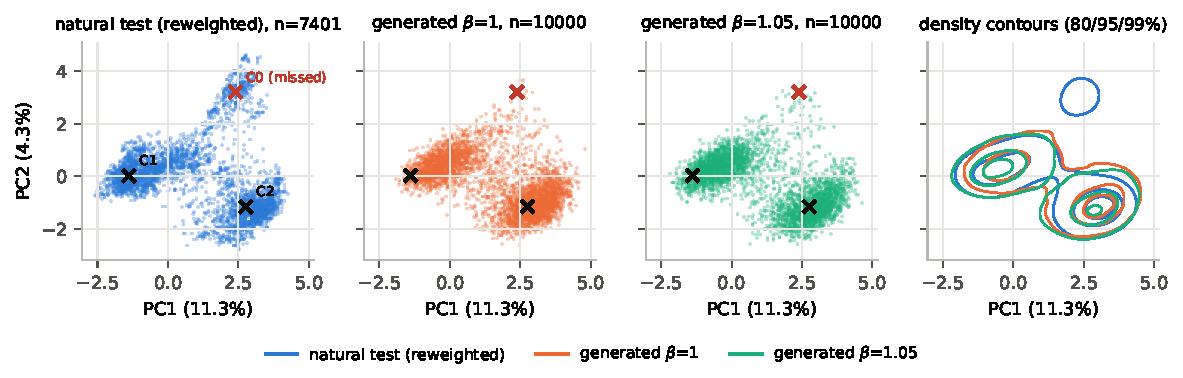
\includegraphics[width=0.86\textwidth]{../outputs/figures/pca_clean.pdf}
\caption{Test and generated sequences on the first two principal components of the one-hot test
alignment (PCA fitted on test only); each panel draws a random sample, the natural panel drawn
with its reweighting weights. Crosses: $k$-means centres, red for the missed cluster.}
\label{fig:pca}
\end{figure*}

\begin{figure*}[t]\centering
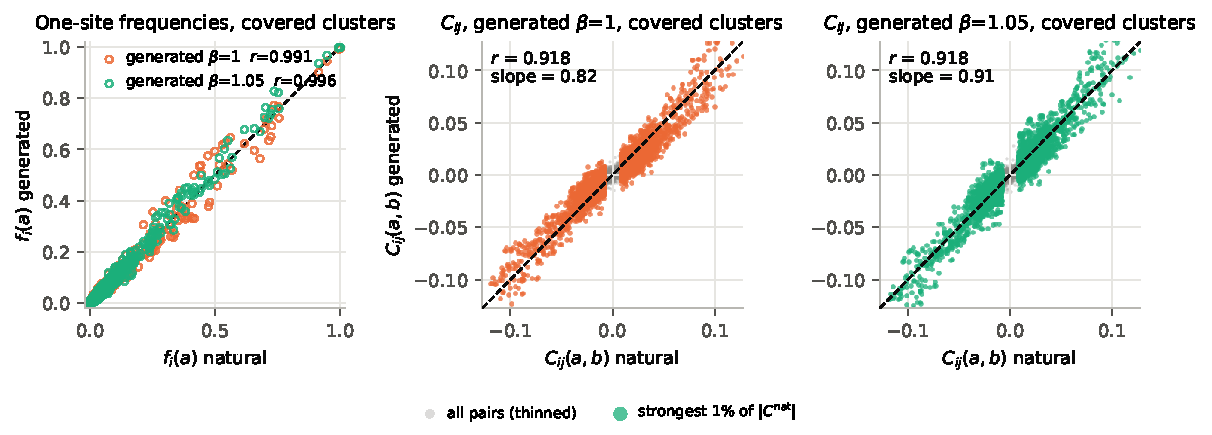
\includegraphics[width=0.86\textwidth]{../outputs/figures/freqs_corr_clusters_clean.pdf}
\caption{As Fig.~\ref{fig:stats}, with natural and generated sets both restricted to the covered
PCA clusters.}
\label{fig:statsclust}
\end{figure*}

\begin{table*}[t]\centering\small\setlength{\tabcolsep}{4pt}
\begin{tabular}{llcccc}
\toprule
statistic & set vs.\ natural (covered clusters) & Pearson $r$ & Spearman $\rho$ & slope & RMSE \\
\midrule
$f_i(a)$ & generated, $\beta=1$ & 0.991 & 0.970 & 0.98 & 0.0153 \\
 & generated, $\beta^*=1.05$ & 0.996 & 0.969 & 1.03 & 0.0118 \\
 & natural train (ceiling) & 0.998 & 0.980 & 0.98 & 0.0079 \\
 & independent-site model & 0.993 & 0.973 & 0.95 & 0.0144 \\
\midrule
$C_{ij}(a,b)$ & generated, $\beta=1$ & 0.918 & 0.179 & 0.82 & 0.0012 \\
 & generated, $\beta^*=1.05$ & 0.918 & 0.199 & 0.91 & 0.0013 \\
 & natural train (ceiling) & 0.941 & 0.345 & 0.87 & 0.0010 \\
 & independent-site model & -0.013 & 0.060 & -0.00 & 0.0031 \\
\midrule
$C_{ij}$, top 1\% & generated, $\beta=1$ & 0.961 & 0.919 & 0.87 & 0.0084 \\
 & generated, $\beta^*=1.05$ & 0.961 & 0.919 & 0.97 & 0.0083 \\
 & natural train (ceiling) & 0.979 & 0.938 & 0.91 & 0.0061 \\
 & independent-site model & -0.031 & -0.035 & -0.00 & 0.0296 \\
\bottomrule
\end{tabular}
\caption{Statistics restricted to the covered PCA clusters (\CovWeight\% of the natural test
weight). Compare Table~\ref{tab:stats}.}
\label{tab:clusters}
\end{table*}

\subsection{The sequences are new, and as diverse as natural ones}
Novelty and diversity are read from three different nearest-neighbour distributions
(Fig.~\ref{fig:ham}, Table~\ref{tab:ham}). Generated sequences sit at \HamGTrOne\ ($\beta=1$) and
\HamGTrStar\ ($\beta^*$) from the closest \emph{training} sequence, whereas a genuine held-out
natural sequence sits at only \HamTestTrain: the model is not reproducing its training set.
All \NgenOne\ samples are distinct (\UniqOne\% unique). Their internal spread, \HamGGOne\ at
$\beta=1$, matches the natural test--test spread of \HamTestTest, and the generated-vs-test
distribution lies on top of it, so the samples neither collapse onto a few modes nor scatter into
regions the family does not occupy. Raising the temperature to $\beta^*$ costs a little of this
diversity (\HamGGStar), which is the price of the corrected correlation amplitude.

Consistently, the energy distribution of the samples at $\beta^*$ overlays the natural one
(Wasserstein distance \WEStar, against \WEOne\ at $\beta=1$ and \WEprof\ for the independent-site
model).

\begin{figure*}[t]\centering
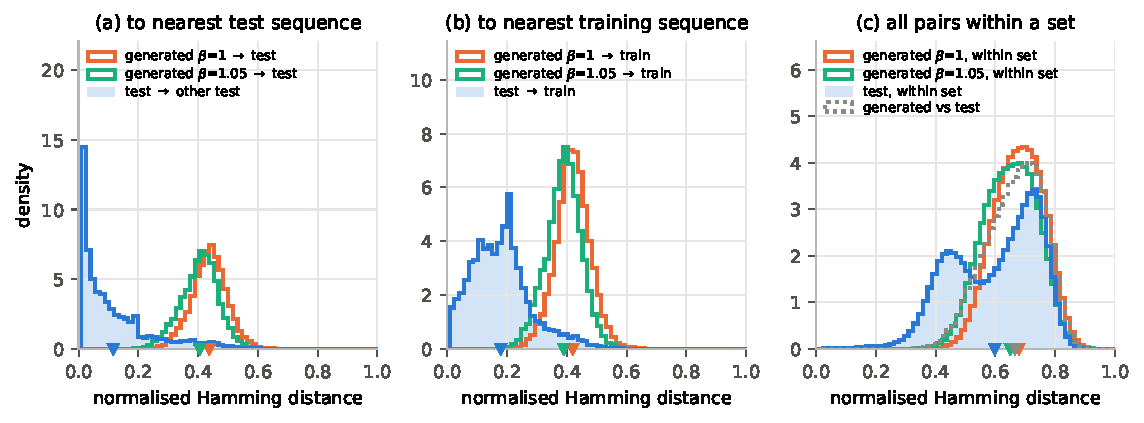
\includegraphics[width=0.92\textwidth]{../outputs/figures/hamming_clean.pdf}
\caption{Normalised Hamming distances; triangles mark means. The blue reference curve is
different in each panel. \textbf{(a)} distance from each sequence to the nearest sequence
\emph{of the natural test set}; blue is a test sequence to its nearest \emph{other} test sequence
(leave-one-out), i.e.\ how close natural relatives normally lie --- its spike near zero is the
family's phylogenetic redundancy. \textbf{(b)} distance to the nearest \emph{training} sequence,
the memorisation check; blue is the held-out test set measured identically, the closest a genuine
unseen J-domain comes to the training data. \textbf{(c)} all pairwise distances \emph{within} one
set (3000 sequences each), i.e.\ the spread of the set itself; blue is the natural test set and
the dotted grey curve is generated-vs-test, which coincides with the generated curve when both
sets occupy the same region of sequence space.}
\label{fig:ham}
\end{figure*}

\begin{table*}[t]\centering\small\setlength{\tabcolsep}{4pt}
\begin{tabular}{lcccc}
\toprule
distance (normalised by $L$) & mean & median & 5\% quantile & $=0$ \\
\midrule
gen ($\beta=1$) $\to$ nearest test & 0.437 & 0.444 & 0.333 & 0.0\% \\
gen ($\beta=1$) $\to$ nearest train & 0.420 & 0.413 & 0.317 & 0.0\% \\
gen ($\beta=1$) $\to$ nearest other gen & 0.430 & 0.429 & 0.349 & 0.0\% \\
gen--gen, all pairs ($\beta=1$) & 0.679 & 0.683 & 0.540 & 0.0\% \\
gen--test, all pairs ($\beta=1$) & 0.666 & 0.683 & 0.492 & 0.0\% \\
\midrule
gen ($\beta^*=1.05$) $\to$ nearest test & 0.405 & 0.413 & 0.302 & 0.0\% \\
gen ($\beta^*=1.05$) $\to$ nearest train & 0.389 & 0.397 & 0.286 & 0.0\% \\
gen ($\beta^*=1.05$) $\to$ nearest other gen & 0.394 & 0.397 & 0.317 & 0.0\% \\
gen--gen, all pairs ($\beta^*=1.05$) & 0.650 & 0.651 & 0.508 & 0.0\% \\
gen--test, all pairs ($\beta^*=1.05$) & 0.639 & 0.651 & 0.460 & 0.0\% \\
\midrule
test $\to$ nearest other test & 0.116 & 0.079 & 0.016 & 0.0\% \\
test $\to$ nearest train & 0.179 & 0.175 & 0.032 & 0.0\% \\
novel test $\to$ nearest train & 0.179 & 0.175 & 0.032 & 0.0\% \\
test--test, all pairs & 0.598 & 0.635 & 0.365 & 0.0\% \\
\bottomrule
\end{tabular}
\caption{Hamming-distance summary; ``$=0$'' is the fraction of exact copies.}
\label{tab:ham}
\end{table*}

%======================================================================
\section{Discussion}
%======================================================================
\paragraph{What the attention parametrisation buys.} With \Nparams\ parameters --- a quarter of
the $861\,273$ entries of a free coupling tensor --- the model reaches near-perfect contact
prediction and a correlation agreement within a few percent of the finite-sample ceiling over
\CovWeight\% of the family. The factorisation is not merely a compression: sharing $V^h$ across
all position pairs is what makes the effective number of parameters small enough for
$M_\text{eff}\approx\MeffTrain$ sequences to constrain.

\paragraph{The $\beta$ offset is a property of pseudo-likelihood, not a bug.} Maximising
Eq.~\eqref{eq:cond} fixes each conditional but leaves the overall scale of $E$ unconstrained, so
there is no reason for the $\beta=1$ chain to sit at the natural energy. The scan of
Fig.~\ref{fig:beta} shows the two failure modes on either side: too low a $\beta$ gives
over-dispersed, weakly correlated samples, too high a $\beta$ collapses diversity. Matching the
mean energy of the training set picks $\beta^*=\BetaStar$ without reference to held-out data and
recovers the correlation amplitude almost exactly.

\paragraph{The missing mode is the substantive limitation.} The under-sampled HscB-like group is
not a sampling artefact --- chains started inside it leave --- but a statement about the learned
landscape: that basin is \EgapMiss\ energy units too shallow, worth \dFmiss\ nats of free energy.
The diagnosis in Table~\ref{tab:clusene} points at the fix, because the failure is in the prior
rather than in the conditionals. Adding explicit fields $h_i$, fitting a mixture over
sub-families, or reweighting the training set towards the minority group would each give the
model somewhere to put that mass; sampling from a mixture of temperatures would paper over it,
since Fig.~\ref{fig:beta} shows the minor cluster is relatively better populated at lower $\beta$.
All are single-parameter experiments on top of the existing pipeline.

\paragraph{On evaluating generative sequence models.} Two methodological points generalise beyond
this family. First, a species-disjoint split is not a sequence-disjoint split; had we not audited
the files, the held-out likelihood would have looked \NLPLgapPct\ percentage points better than it
is. Second, aggregate correlation scores conflate ``distorts the covariation'' with ``misses a
sub-family''. Partitioning the family and re-scoring inside the covered modes separates the two,
and here it moves the interpretation from ``the model captures 87\% of the correlation structure''
to ``the model is near the sampling limit on \CovWeight\% of the family and misses the rest''.
Those are different problems with different fixes.

%======================================================================
\section{Conclusion}
%======================================================================
An attention-parametrised Potts model trained by pseudo-likelihood on \Mtrain\ bacterial
J-domains generates sequences that are new, as diverse as natural ones, and statistically
faithful over the bulk of the family: $r=\rFOne$ on site frequencies, $r=\rCOne$ on connected
correlations, rising to $\rCcovOne$ against a $\rCtrainCov$ ceiling on the modes the sampler
populates. The residual error is concentrated in one under-weighted sub-family rather than spread
over the covariation structure, and the sampler itself is fast (${\sim}0.3\,\mu$s per
chain-update) and well-mixed ($\tau_\text{int}=\TauOne$ sweeps).

\vspace{0.3cm}
\noindent\small
Code: \texttt{attdca/} (package), \texttt{scripts/} (pipeline), \texttt{tests/} (vectorised
likelihood, energy, sampler and split checked against naive loops and an exact two-site Gibbs
target). A longer companion report documents the derivations and the full metric definitions.

\end{document}
